\documentclass[aspectratio=169]{beamer}
\usetheme{Madrid}
\usecolortheme{default}
\usepackage{amsmath}
\usepackage{amssymb}
\usepackage{bbding}
\usepackage{tikz}
\title{Black Holes and Entropy}
\subtitle{A presentation on the paper by Jacob D. Bekenstein}
\author{Advik Adatiya, Ashish Paul and Chinmay Wasnik}
\date{October 17, 2026}

\begin{document}

\begin{frame}
    \titlepage
\end{frame}

\begin{frame}{Introduction}
  \begin{columns}
    \begin{column}{0.65\textwidth}
          \begin{itemize}
            \item \textit{Floyd \& Penrose (1971):} Horizon area increases in energy extraction processes.
            \item \textit{Christodoulou (1970):} $dM_{\text{ir}} \ge 0$ for Kerr black holes.
        \item \textbf{Hawking's Area Theorem (1971):} $\Delta A \ge 0$
        \item \textbf{The Analogy:}
          \begin{itemize}
            \item Both black hole area ($A$) and thermodynamic entropy ($S$) increase irreversibly in closed systems.
            \item \textbf{Goal:} Unify black hole physics with classical thermodynamics.
          \end{itemize}
      \end{itemize}
    \end{column}
    
    \begin{column}{0.35\textwidth}
      \begin{block}{Irreducible Mass}
        \begin{equation*}
          M_{\text{ir}} = \sqrt{\frac{A}{16\pi}}
        \end{equation*}
        Represents degraded energy that cannot be extracted via the Penrose process.
      \end{block}
    \end{column}
  \end{columns}
\end{frame}

\begin{frame}{Thermodynamic Analogies}
\framesubtitle{Rationalized Horizon Area}
\begin{column}{0.4\textwidth}
    \begin{block}{}
     Define rationalized area $\alpha \equiv \frac{A}{4\pi}$. \\ For a Kerr-Newman black hole of $M$, $Q$ and $\vec{L}$:
    \begin{equation*}
      \alpha = r_+^2 + a^2 = 2Mr_+ - Q^2 \quad \\ \text{where: } \\ r_\pm = M \pm \sqrt{M^2 - Q^2 - a^2}, \quad \vec{a} = \frac{\vec{L}}{M}
    \end{equation*}
    \end{block} 
   \end{column}
    \begin{column}{0.6\textwidth}
    \begin{center}
        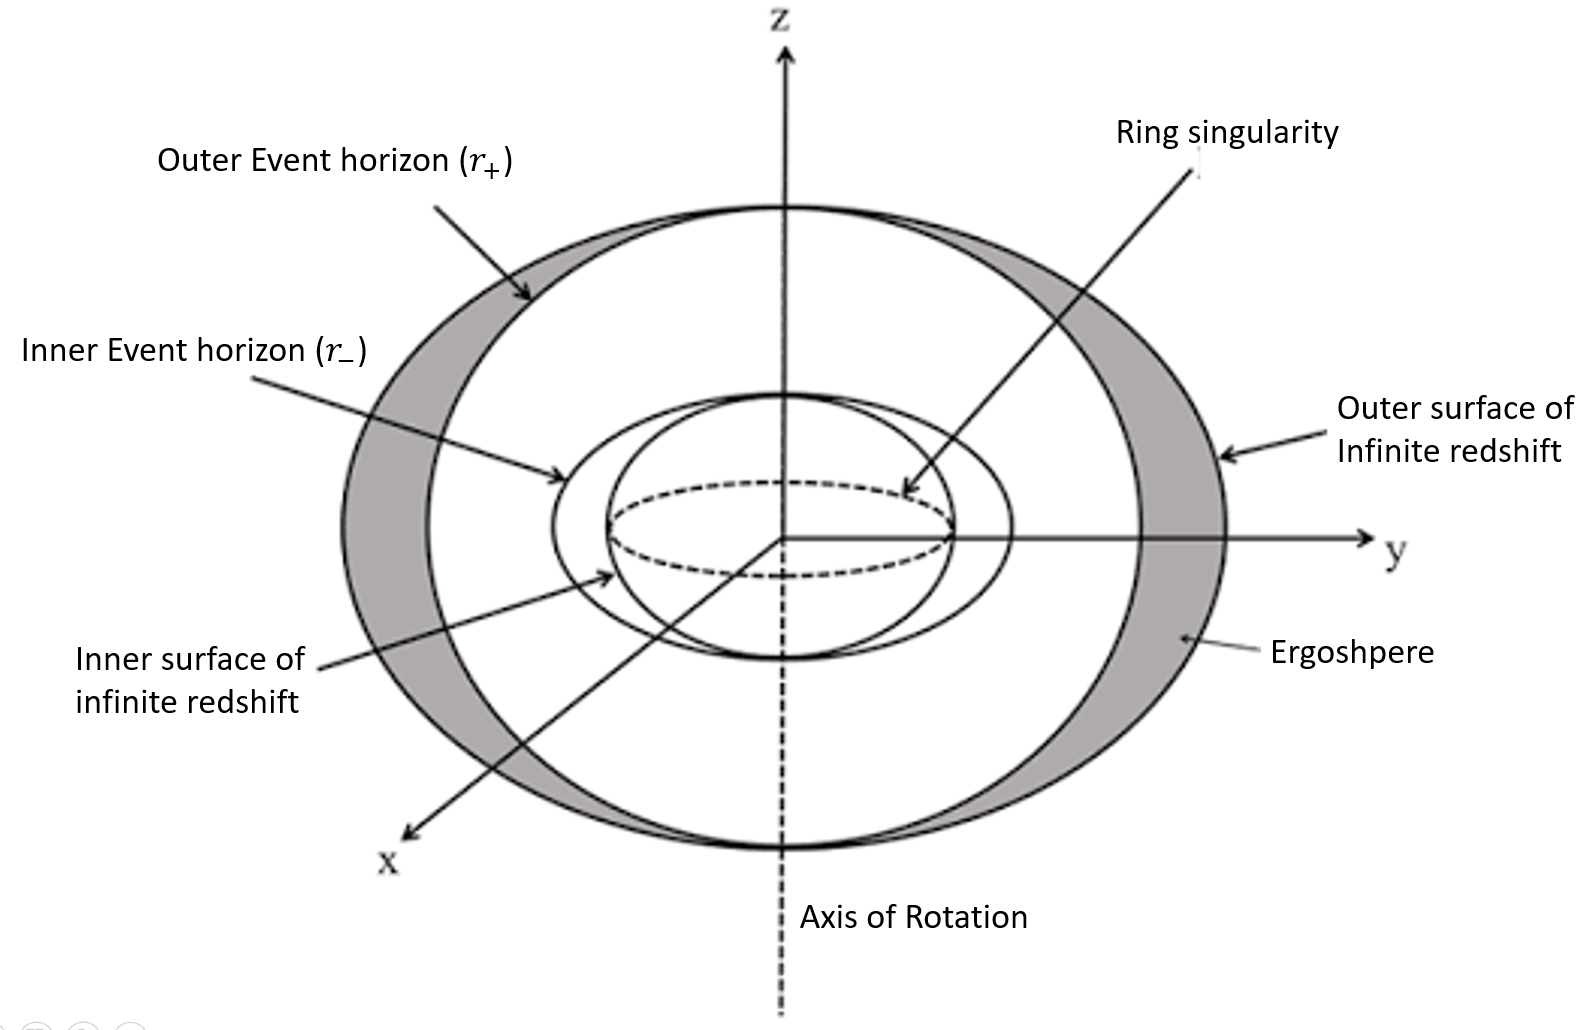
\includegraphics[width=0.9\textwidth]{image.png}
    \end{center}
    \end{column}
\end{frame}

\begin{frame}{Thermodynamic Analogies}
\framesubtitle{Differential Mass Formula ($dM$)}
Differentiating $\alpha$ and solving for $dM$ yields:
    \begin{equation*}
      \boxed{dM = \Theta d\alpha + \vec{\Omega} \cdot d\vec{L} + \Phi dQ}
    \end{equation*}
      \begin{itemize}
    \item \textbf{Effective Temperature Factor ($\Theta$):} $\Theta \equiv \frac{1}{4} \frac{r_+ - r_-}{\alpha}$
    \item \textbf{Rotational Angular Frequency ($\vec{\Omega}$):} $\vec{\Omega} \equiv \frac{\vec{a}}{\alpha}$
    \item \textbf{Electric Potential ($\Phi$):} $\Phi \equiv \frac{Q r_+}{\alpha}$
  \end{itemize}
\end{frame}

\begin{frame}{Thermodynamic Analogies}
\framesubtitle{Comparison with First Law of Thermodynamics}
  \begin{table}[h]
    \centering
    \begin{tabular}{|l|c|c|}
      \hline
      \textbf{Physical Quantity} & \textbf{Thermodynamics} & \textbf{Black Hole Mechanics Equivalent} \\
      \hline\hline
      First Law Equation & $dE = T dS - P dV$ & $dM = \Theta d\alpha + \vec{\Omega} \cdot d\vec{L} + \Phi dQ$ \\
      \hline
      Energy & $E$ & $M$ \\
      \hline
      Entropy & $S$ ($dS \ge 0$) & $\alpha$ ($d\alpha \ge 0$) \\
      \hline
      Temperature & $T \ge 0$ & $\Theta \ge 0$ \\
      \hline
      Work Terms & $-P dV$ & $\vec{\Omega} \cdot d\vec{L} + \Phi dQ$ \\
      \hline
    \end{tabular}
  \end{table}

  \vspace{0.3cm}
  \begin{alertblock}{Note:}
    Purely formal analogy so far due to mismatched dimensions ($\alpha$ is length$^2$, $S$ is dimensionless).
  \end{alertblock}
\end{frame}

\begin{frame}{Information Theory \& Black Hole Entropy}
\framesubtitle{Entropy as Missing Information}
   \begin{itemize}
        \item Shannon entropy measures lack of information about a system's internal state:
          \begin{equation*}
            S = -\sum_n p_n \ln p_n \quad \implies \quad \Delta I = -\Delta S
          \end{equation*}
        \item Units are in "bits". $1\text{ bit} = \ln 2$, the maximum entropy of a yes/no question ($p_{\text{yes}} = p_{\text{no}} = \tfrac12$).
    \end{itemize}
\end{frame}

\begin{frame}{Information Theory \& Black Hole Entropy}
\framesubtitle{Black Holes as Thermodynamic Systems}
    \begin{itemize}
        \item An exterior observer knows only 3 macro-parameters: $M$, $Q$, and $\vec{L}$.
        \item The inaccessible internal configurations are measured by Black hole entropy ($S_{\text{bh}}$).
        \item Now, we postulate a general equation for $S_{\text{bh}}$
          \begin{equation*}
            S_{\text{bh}} = f(\alpha) \text{, monotonically increasing}
          \end{equation*}
    \end{itemize}
    \textbf{Why this is sensible:}
    \begin{enumerate}
        \item $d\alpha \ge 0$: According to Hawking
        \item $dS_{\text{bh}} \ge 0$: The one-way horizon prevents an outside agent from learning the interior.
    \end{enumerate}
\end{frame}

% Slide: Ruling out f(\alpha) \propto \alpha^{1/2}
\begin{frame}{Information Theory \& Black Hole Entropy}
\framesubtitle{Finding $f(\alpha)$}
  
  \begin{itemize}
    \item Consider two distant, weakly interacting black holes that fall together and merge.
    \item \textbf{Condition:} $S_{\text{final}} \ge S_1 + S_2$
    \item Let $f(\alpha) \propto \alpha^{n}$
  \end{itemize}
  \begin{enumerate}
        \item $n < 1$ \XSolidBrush \\
        Example: $f(\alpha) \propto \alpha^{\frac{1}{2}}$   \\
        Contradiction: 
        \begin{itemize}
            \item $f(\alpha) \propto \alpha^{\frac{1}{2}} \propto M_{\text{ir}}$
            \item For Schwarzschild black holes, $M_{\text{ir}} = M$. Then, $M_{\text{final}} \ge M_1 + M_2$
        \end{itemize}
        \item $n \ge 1$ \Checkmark \\
        Correct solution: $f(\alpha) \propto \alpha$ 
    \end{enumerate}
\end{frame}

%% ------------------------------------------------------------
%% Timing guide (total approx. 4:30)
%%  1 Bridge ~25s | 2 Setup S=f(alpha) ~40s | 3 One bit ~40s | 4 Min. area ~40s
%%  5 Quantum bound ~40s | 6 Result ~35s | 7 Consequences ~40s

%% ---------- 4. ONE BIT ----------
\begin{frame}{Information Theory \& Black Hole Entropy}
\framesubtitle{Fixing the Constant, with a Particle Falling In}
$f(\alpha) \propto \alpha \implies S_{\text{bh}} = \eta\,\hbar^{-1}\alpha$, with $\eta$ a dimensionless constant of order unity. Goal: find $\eta$.

\vspace{4pt}
\textbf{Idea:} drop a particle into a Kerr black hole and ask how much information is lost with it.
\begin{itemize}
  \item Before: we know the answer to ``does the particle exist?'' is \emph{yes}.
  \item After it falls in: we know nothing about the physical conditions inside, so we have no information about that answer.
  \item So, \textbf{at least one bit} is lost, and one bit $=\ln 2$, as shown earlier.
\end{itemize}
\begin{alertblock}{Plan}
Minimum area increase $\Delta\alpha_{\min}$ $\;\Rightarrow\;$ minimum entropy increase $\;\Rightarrow\;$ set it equal to $\ln 2$.
\end{alertblock}
\end{frame}

%% ---------- 5. MIN AREA ----------
\begin{frame}{Expression for Black Hole Entropy}
\framesubtitle{Smallest Possible Area Increase}
\begin{itemize}
  \item \textbf{Christodoulou:} a freely falling \emph{point} particle captured from a turning point of its orbit leaves $\Mir$ and the area unchanged: $\Delta\alpha = 0$.
  \item \textbf{Generalization:} let the particle have rest mass $\mu$ and nonzero proper radius $b$. It must be captured with its centre a proper distance $b$ outside the horizon.
\end{itemize}
\begin{block}{Result}
\[
  (\Delta\alpha)_{\min} = 2\mu b
\]
independent of $M$, $Q$ and $\vec L$ of the black hole. For a point particle ($b\to 0$) it reduces to Christodoulou's $0$.
\end{block}
Can we make it arbitrarily small by shrinking $b$? Not once quantum effects are included.
\end{frame}

%% ---------- 6. QUANTUM BOUND ----------
\begin{frame}{Expression for Black Hole Entropy}
\framesubtitle{Quantum Lower Bound on the Area Increase}
The radius $b$ cannot be smaller than the particle's
\[
  \text{Compton wavelength } \frac{\hbar}{\mu}
  \quad\text{or its gravitational radius } 2\mu,
  \quad\text{whichever is larger.}
\]
\begin{columns}[T]
\begin{column}{0.49\textwidth}
\textbf{If} $\mu \lesssim 2^{-1/2}\hbar^{1/2}$ (Compton larger):
\[
  2\mu b \;\ge\; 2\mu\cdot\frac{\hbar}{\mu} = 2\hbar
\]
\end{column}
\begin{column}{0.49\textwidth}
\textbf{If} $\mu > 2^{-1/2}\hbar^{1/2}$ (gravitational radius larger):
\[
  2\mu b \;\ge\; 4\mu^{2} > 2\hbar
\]
\end{column}
\end{columns}
\vspace{4pt}
\begin{block}{Conclusion}
Quantum effects set $(\Delta\alpha)_{\min} = 2\hbar$, reached only by an elementary particle of Compton size. Such a particle has no internal structure, so it loses the least information. This supports identifying $2\hbar$ with the loss of \textbf{one bit}.
\end{block}
\end{frame}

%% ---------- 7. RESULT ----------
\begin{frame}{Expression for Black Hole Entropy}
Equate the minimum entropy increase with one bit:
\[
  (\Delta S_{\text{bh}})_{\min} = 2\hbar\,\frac{df}{d\alpha} = \ln 2
  \quad\Longrightarrow\quad
  \boxed{\;S_{\text{bh}} = \tfrac12\ln 2\;\hbar^{-1}\,\alpha\;}
\]
so $\eta = \tfrac12 \ln 2$. In conventional units:
\[
  S_{\text{bh}} = \frac{\ln 2}{8\pi}\,\frac{k c^{3}}{\hbar G}\,A
  = \left(1.46\times10^{48}\ \mathrm{erg\,K^{-1}\,cm^{-2}}\right)A
\]
\begin{itemize}
  \item Caveat: this assumes a particle's smallest radius is \emph{exactly} its Compton wavelength, which is not sharply defined. So $\eta$ is only fixed to within about a factor of two. The price of a semiclassical treatment.
  \item Later examples show this value leads to no contradictions.
\end{itemize}
\end{frame}

%% ---------- 8. CONSEQUENCES ----------
\begin{frame}{Expression for Black Hole Entropy}
\framesubtitle{Consequences}
\begin{itemize}
  \item \textbf{Enormous magnitude:} a one-solar-mass black hole has $S_{\text{bh}} \approx 10^{60}\ \mathrm{erg\,K^{-1}}$, versus $\approx 10^{42}$ for the Sun; a white dwarf or neutron star of the same mass has even less. This dramatizes how irreversible black-hole formation is.
  \item \textbf{Characteristic temperature:} from $T_{\mathrm{bh}}^{-1} = \partial S_{\text{bh}}/\partial M$ and $dM = \Theta\,d\alpha+\dots$
  \[
    T_{\mathrm{bh}} = 2\hbar\,(\ln 2)^{-1}\,\Theta
  \]


\end{itemize}
\end{frame}
% ============================================================
% Section V: The Generalized Second Law
% Paste after the "Consequences" slide and before
% \section{Testing the Generalized Second Law}
% Builds on: Shannon entropy slide (Delta I = -Delta S),
%            S_bh = f(alpha) slides, Hawking's area theorem,
%            "Several black holes" bullet on the Consequences slide.
% ============================================================

\begin{frame}{Generalized Second Law}
\framesubtitle{A Puzzle: Entropy Falling into a Black Hole}
\begin{itemize}
  \item \textbf{Puzzle:} drop a body with entropy $S$ into a black hole. The entropy of the outside universe drops, $\Delta S_c = -S$.
  \item An outside observer can never check that total entropy did not decrease. Is the second law \emph{transcended}?
  \item \textbf{Resolution:} recall $\Delta I = -\Delta S$. Before the fall, we could measure the body and recover information $S$. After the fall, that option is gone.
  \item So $S_{\text{bh}}$ must grow by \textbf{at least} $S$. The area ``compensates''.
\end{itemize}
\begin{block}{Generalized Second Law (GSL)}
\centering
The entropy outside plus the black hole entropy never decreases:
\[
  \Delta S_{\text{bh}} + \Delta S_c \ge 0
\]
\end{block}
\end{frame}


% ============================================================
% Section: Testing the Generalized Second Law (Secs. VI & VII)
% (Assumes preceding slides already introduced S_bh, GSL, etc.)
% ============================================================

% ============================================================
% Section: Testing the Generalized Second Law (Secs. VI & VII)
% (Assumes preceding slides already introduced S_bh, GSL, etc.)
% Includes intermediate derivation steps (p_n, bounds, etc.)
% ============================================================

% ============================================================
% Section: Testing the Generalized Second Law (Secs. VI & VII)
% (Assumes preceding slides already introduced S_bh, GSL, etc.)
% ============================================================

% ============================================================
% Section: Testing the Generalized Second Law (Secs. VI & VII)
% (Assumes preceding slides already introduced S_bh, GSL, etc.)
% ~5 min budget: Geroch process (priority) + Harmonic oscillator.
% No intermediate derivations -- results only.
% ============================================================
% ============================================================
% Section: Testing the Generalized Second Law (Secs. VI & VII)
% (Assumes preceding slides already introduced S_bh, GSL, etc.)
% ~5 min budget: Geroch process (priority, paradox shown explicitly)
% + Harmonic oscillator. No intermediate derivations elsewhere.
% ============================================================

\section{Testing the Generalized Second Law}

\begin{frame}{Strategy}
\begin{itemize}
    \item GSL claims: $\Delta S_{\rm bh}+\Delta S_c \ge 0$ for \textbf{any} process.
    \item We test it on two worst-case examples:
    \begin{enumerate}
        \item A harmonic oscillator in a box
        \item Geroch's box-lowering heat engine
    \end{enumerate}
    \item Each case tries to maximize entropy in / minimize area increase.
\end{itemize}
\end{frame}

% % ---------------------------------------------------
\begin{frame}{Example 1: Harmonic Oscillator in a Box}
Two masses $\tfrac12 m$, spring const.\ $K=\tfrac14 m\omega^2$, in a box, temperature $T$.

\vspace{0.2cm}
\textbf{Canonical distribution}, $x\equiv\hbar\omega/T$:
\[
p_n=(1-e^{-x})e^{-nx}
\]
\[
S = \frac{x}{e^x-1} - \ln(1-e^{-x}),
\qquad
\langle E\rangle = \hbar\omega\left(\frac{1}{e^x-1}+\tfrac12\right)
\]

\vspace{0.15cm}
\textbf{Box size:} must satisfy $b \gtrsim \tfrac12\,\Delta y_{\rm rms}$ — the box has to physically contain the particles' thermal (rms) spread $\Delta y$, else they wouldn't fit. Virial theorem then gives
\[
b \gtrsim \langle E\rangle^{1/2}\,m^{-1/2}\,\omega^{-1}
\]


\begin{center}
\[
\boxed{\;\Delta S_{\rm bh} \;\ge\; \mu\, b\,\hbar^{-1}\ln 2\;}, \qquad \mu > m+\langle E\rangle
\]
\end{center}
\vspace{0.1cm}
\end{frame}

% ---------------------------------------------------
\begin{frame}{Result}
Combine everything, $\xi \equiv m/\langle E\rangle$:
\[
\Delta(S_{\rm bh}+S_c) > \xi^{-1/2}(1+\xi)\Big[\tfrac12+(e^x-1)^{-1}\Big]\ln2 - \frac{x}{e^x-1}+\ln(1-e^{-x})
\]
Minimizing over $x$: stationary point at
\[
x_m = \xi^{-1/2}(1+\xi)\ln 2
\]
\[
\Delta(S_{\rm bh}+S_c)\Big|_{\min} = \tfrac12 x_m + \ln\!\big(1-e^{-x_m}\big) \; > \;0 \quad (\xi \gg 1)
\]
\centering
\textbf{Second law holds} for the non-relativistic oscillator.
\end{frame}

\begin{frame}{Example 2: Geroch's Process}
\begin{columns}[c]
\column{0.48\textwidth}
\begin{center}
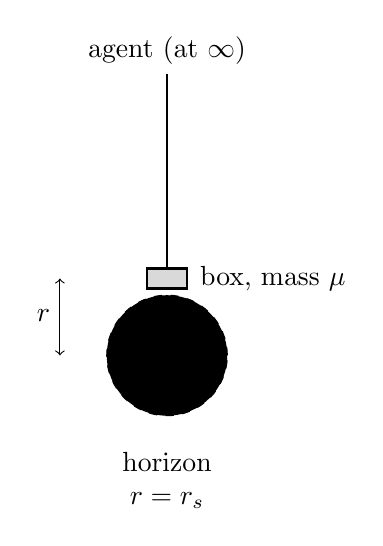
\begin{tikzpicture}[scale=0.85]
    % black hole
    \fill[black] (0,0) circle (0.9);
    \draw[dashed] (0,0) circle (0.9)
        node[below=1.1cm, align=center] {horizon\\$r=r_s$};
    % string from infinity
    \draw[thick] (0,4.2) -- (0,1.3);
    \node[above] at (0,4.2) {agent (at $\infty$)};
    % box near horizon
    \draw[fill=gray!30, thick] (-0.3,1.0) rectangle (0.3,1.3);
    \node[right] at (0.35,1.15) {box, mass $\mu$};
    % radius arrow
    \draw[<->, thin] (-1.6,0) -- (-1.6,1.15);
    \node[left] at (-1.6,0.6) {$r$};
\end{tikzpicture}
\end{center}

\column{0.48\textwidth}
Box of radiation (mass $\mu$) lowered on a string to radius $r$ near the horizon.

\vspace{0.3cm}
Energy as measured \textbf{from infinity} (gravitational redshift):
\[
E(r) = \mu\,c^2\sqrt{1-\dfrac{r_s}{r}}
\]

\vspace{0.3cm}
As the box approaches the horizon, $r\to r_s^+$:
\[
\boxed{E(r)\;\longrightarrow\;0}
\]
\end{columns}
\end{frame}

\begin{frame}{The Naive Cycle: Heat Engine at the Horizon}
Operate a cyclic heat engine between infinity and radius $r$:
\begin{itemize}
    \item \textbf{Lower} mass $\mu$: winch extracts work $W_{\text{down}} = \mu - E(r)$
    \item \textbf{Dump} heat $\Delta\mu$ into the hole at radius $r$
    \item \textbf{Hoist} remaining mass $(\mu - \Delta\mu)$
\end{itemize}

\vspace{0.3cm}
Net work extracted per cycle:
\[
W_{\text{net}} = W_{\text{down}} - W_{\text{up}} = \Delta\mu \left(1 - \sqrt{1 - \frac{r_s}{r}}\right)
\]

\vspace{0.3cm}
In the naive point-particle limit ($r \to r_s$):
\[
\boxed{\epsilon = \frac{W_{\text{net}}}{\Delta\mu} \;\longrightarrow\; 1}
\]
\begin{itemize}
    \item Directly violates the Kelvin--Planck statement of the 2nd Law.
\end{itemize}
\end{frame}

\begin{frame}{The Flaw: Accounting for Finite Size}
\textbf{Why the naive limit fails:}
\begin{itemize}
    \item A thermal box cannot be a mathematical point ($b \to 0$).
    \item Center of mass is halted at proper distance $b$ outside the horizon.
\end{itemize}

\vspace{0.3cm}
\textbf{Determining the cutoff energy (from earlier slides):}
\begin{itemize}
    \item Minimum area increase for a body of size $b$:
    \[
    (\Delta\alpha)_{\min} = 2\mu b
    \]
    \item First Law of black hole mechanics :
    \[
    dM = \Theta\,d\alpha \implies E = \Theta(\Delta\alpha)
    \]
\end{itemize}

\vspace{0.2cm}
Energy delivered to the black hole at closest approach:
\[
\boxed{E = 2\mu b\,\Theta}
\]
\end{frame}

% \begin{frame}{The Corrected Efficiency Bound}
% Replacing the coordinate redshift with the physical cutoff $2b\Theta$:

% \vspace{0.2cm}
% Net work extracted per cycle:
% \[
% W_{\text{net}} = \Delta\mu(1 - 2b\,\Theta)
% \]

% \vspace{0.2cm}
% True conversion efficiency:
% \[
% \boxed{\epsilon = 1 - 2b\,\Theta}
% \]

% \vspace{0.4cm}
% \textbf{The Remaining Threat:}
% \begin{itemize}
%     \item If $b$ could be made arbitrarily small ($b \to 0$), then $\epsilon \to 1$.
%     \item To save the 2nd Law, \textbf{quantum mechanics must set a lower bound on $b$}[cite: 10, 30].
% \end{itemize}
% \end{frame}
\begin{frame}{The Paradox: Efficiency $\to 1$}
Energy of the box, as measured from infinity, at the horizon:
\[
E = 2\mu b\,\Theta
\]

Replacing the coordinate redshift with the physical cutoff $2b\Theta$:

\vspace{0.2cm}
Net work extracted per cycle:
\[
W_{\text{net}} = \Delta\mu(1 - 2b\,\Theta)
\]
This gives a net conversion efficiency of
\[
\boxed{\epsilon = 1-2b\,\Theta}
\]
\begin{itemize}
    \item If $b\to 0$: $\;\epsilon \to 1$ — a \textbf{perfect} heat-to-work converter!
    \item Forbidden by the ordinary 2nd law — \textbf{something must stop $b$ from shrinking to zero.}
\end{itemize}
\end{frame}
\begin{frame}{The Resolution}
\begin{columns}[c]
\column{0.55\textwidth}
\begin{itemize}
    \item A box can't hold well-defined radiation at temperature $T$ unless it's big enough to contain the relevant thermal wavelengths.
    % \item Longest wavelength that fits: $\lambda_{\max}/2 \approx 2b \;\Rightarrow\; \omega_{\min} \approx \pi/2b$.
    \item Requiring this to still match the thermal spectrum at $T$ gives an \textbf{independent, quantum-mechanical} inequality for $b$ — a strict lower bound:
    \[
    \boxed{b > \frac{\pi\hbar}{2T}}
    \]
    \item So $b$ can \textbf{never} actually be shrunk to zero.
\end{itemize}

\column{0.43\textwidth}
\centering
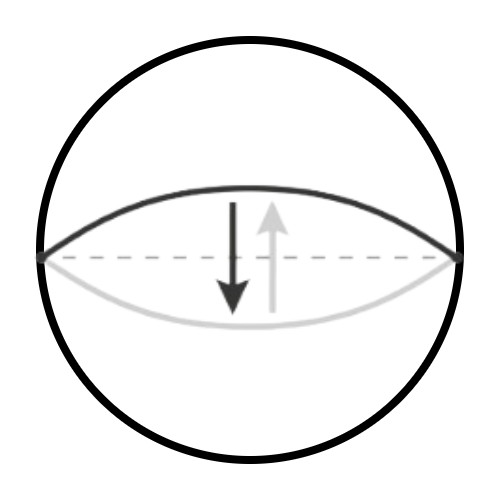
\includegraphics[width=0.4\textwidth]{overlay-image (2).jpg}

\vspace{0.1cm}
{\footnotesize $\lambda_{\max}/2 \approx 2b \;\Rightarrow\; \omega_{\min} \approx \pi/2b$.}

\vspace{0.25cm}
% --- Planck Spectrum & Cutoff Mode Illustration ---
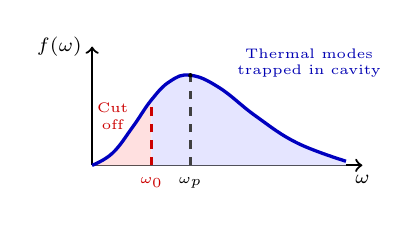
\begin{tikzpicture}[scale=0.52]
    % Axes
    \draw[->, thick] (0,0) -- (6.6,0) node[below, font=\scriptsize] {$\omega$};
    \draw[->, thick] (0,0) -- (0,2.9) node[left, font=\scriptsize] {$f(\omega)$};

    % Forbidden zone: omega < omega_0 (shaded light red)
    \fill[red!12] (0,0) 
        -- plot[smooth, tension=0.7] coordinates {(0,0) (0.5,0.3) (1.0,0.95) (1.45,1.6)} 
        -- (1.45,0) -- cycle;

    % Allowed cavity modes: omega >= omega_0 (shaded light blue)
    \fill[blue!10] (1.45,0) -- (1.45,1.6) 
        -- plot[smooth, tension=0.7] coordinates {(1.45,1.6) (1.9,2.05) (2.4,2.2) (3.1,1.9) (4.0,1.2) (5.0,0.55) (6.2,0.1)} 
        -- (6.2,0) -- cycle;

    % Planck spectrum curve
    \draw[very thick, blue!75!black] plot[smooth, tension=0.7] coordinates {
        (0,0) (0.5,0.3) (1.0,0.95) (1.45,1.6) (1.9,2.05) (2.4,2.2) (3.1,1.9) (4.0,1.2) (5.0,0.55) (6.2,0.1)
    };

    % Cutoff frequency line (omega_0)
    \draw[thick, dashed, red!80!black] (1.45,0) -- (1.45,1.6);
    \node[below, red!80!black, font=\tiny] at (1.45,-0.05) {$\omega_0$};

    % Planck peak line (omega_p)
    \draw[thick, dashed, darkgray] (2.4,0) -- (2.4,2.2);
    \fill[black] (2.4,2.2) circle (1.5pt);
    \node[below, font=\tiny] at (2.4,-0.05) {$\omega_p$};

    % % Inset condition arrow
    % \draw[<->, >=stealth, thin, darkgray] (1.45, 0.5) -- (2.4, 0.5)
    %     node[midway, above, font=\tiny] {$\omega_0 \le \omega_p$};

    % Region labels
    \node[red!80!black, font=\tiny, align=center] at (0.5, 1.2) {Cut\\off};
    \node[blue!70!black, font=\tiny, align=center] at (5.3, 2.5) {Thermal modes\\trapped in cavity};
\end{tikzpicture}
\end{columns}
\end{frame}


\begin{frame}{Result: The Carnot Bound Emerges}
Substituting this minimum $b$ back into $\epsilon = 1-2b\Theta$:
\[
\boxed{\epsilon < 1-\frac{T_{\rm bh}}{T}}
\]
\begin{itemize}
    \item Exactly the \textbf{Carnot efficiency} for a reservoir at $T_{\rm bh}$.
    \item The black hole behaves like an ordinary finite-temperature heat sink, \textbf{not} a perfect one.
    \item Checked independently via direct entropy bookkeeping — same conclusion: $\Delta(S_{\rm bh}+S_c)>0$.
\end{itemize}
\centering
\textbf{No violation. No perpetual motion.}
\end{frame}

% ============================================================
% \subsection{Harmonic Oscillator in a Box}

% \begin{frame}{Setup}
% Two masses on a spring, enclosed in a box, temperature $T$, lowered into the hole.
% \begin{itemize}
%     \item Oscillator carries thermal entropy $S(x)$, energy $\langle E\rangle(x)$, where $x=\hbar\omega/T$.
%     \item Virial theorem fixes the minimum box radius $b$ needed to contain it.
%     \item GR tells us how much $\Delta S_{\rm bh}$ this guarantees once lowered in.
% \end{itemize}
% \end{frame}

% \begin{frame}{Result:}
% Minimizing $\Delta(S_{\rm bh}+S_c)$ over all possible oscillator temperatures $x$:
% \[
% \Delta(S_{\rm bh}+S_c)\Big|_{\min} > 0 \qquad \text{(for a non-relativistic oscillator)}
% \]
% \begin{itemize}
%     \item Even in the \textbf{worst case} — maximum entropy dumped, minimum area gained — the law survives.
%     \item Holds for \emph{any} non-relativistic oscillator, any temperature.
% \end{itemize}
% \end{frame}

% ============================================================
\begin{frame}{Summary}
\begin{itemize}
    \item \textbf{Geroch engine:} the paradox ($\epsilon\to1$) is resolved by a quantum limit on box size — efficiency is capped at the Carnot bound.
    \item \textbf{Oscillator:} worst-case entropy balance stays positive for any non-relativistic oscillator.
\end{itemize}
\centering
\textbf{In both cases: } $\Delta S_{\rm bh}+\Delta S_c \ge 0$ — the Generalized Second Law holds.
\end{frame}

% Slide: Conclusion & Summary of Key Results
\begin{frame}{Conclusion and Summary}
    \begin{block}{First Law of BH Mechanics}
        \begin{equation*}
          dM = \Theta d\alpha + \vec{\Omega} \cdot d\vec{L} + \Phi dQ
        \end{equation*}
    \end{block}
    \begin{block}{Bekenstein-Hawking Entropy}
        \begin{equation*}
          S_{\text{bh}} = \left(\frac{1}{2} \ln 2\right) \hbar^{-1} \alpha = \left(\frac{\ln 2}{8\pi}\right) \frac{k c^3}{\hbar G} A
        \end{equation*}
    \end{block}
    \begin{block}{Generalized Second Law (GSL)}
         \begin{equation*}
          \Delta S_{\rm bh}+\Delta S_c \ge 0
        \end{equation*}
    \end{block}
\end{frame}
% ============================================================
% APPENDIX SLIDES
% ============================================================
\appendix

% Slide 1: Assumptions of (\Delta\alpha)_min = 2\mu b
\begin{frame}{Appendix: Assumptions for $(\Delta\alpha)_{\min} = 2\mu b$}
\framesubtitle{Physical and Kinematic Conditions (Paper Appendix A)}

\begin{columns}[T]
\begin{column}{0.48\textwidth}
  \begin{block}{Particle \& Capture State}
  \begin{itemize}
    \item \textbf{Isolated \& Neutral:} Spherical particle (mass $\mu$, proper radius $b$), zero charge, ignoring incidental radiation.
    \item \textbf{Boundary Condition:} Captured exactly at a proper distance $b$ outside the event horizon ($r = r_+ + \delta$).
    \item \textbf{Geodesic Motion:} Particle is in pure free fall at the precise moment of capture.
  \end{itemize}
  \end{block}
\end{column}

\begin{column}{0.48\textwidth}
  \begin{block}{Energy Minimization \& Math}
  \begin{itemize}
    \item \textbf{Zeroed Momentum:} To minimize energy, the particle is captured at a radial turning point ($p^r = 0$) with zero angular momentum ($p_\theta = p_\phi = 0$).
    \item \textbf{First-Order Expansion:} Energy is expanded to $O(b)$, assuming the particle is vastly smaller than a non-extreme black hole.
  \end{itemize}
  \end{block}
  
  \vspace{0.2cm}

\end{column}
\end{columns}
\end{frame}
% Slide 2: Uniqueness of f(\alpha) \propto \alpha (Differential Equation)
\begin{frame}{Appendix: Why $S_{\text{bh}} = f(\alpha)$ Must Be Strictly Linear}
\framesubtitle{The Differential Proof from Information Theory (Section IV)}
\begin{itemize}
  \item \textbf{Universal Area Gain:} An elementary particle has minimum radius $b = \hbar/\mu$ (Compton wavelength), yielding an absolute universal lower bound:
  \[
    (\Delta\alpha)_{\min} = 2\mu\left(\frac{\hbar}{\mu}\right) = 2\hbar \quad (\text{independent of } \alpha, M, Q, \vec{L})
  \]
  \item \textbf{Universal Information Loss:} Swallowing an elementary particle without internal structure destroys exactly \textbf{1 bit} ($=\ln 2$) of accessible information.
  \item \textbf{Calculus Constraint:} Relating the minimum variations:
  \[
    (\Delta S_{\text{bh}})_{\min} = \frac{df}{d\alpha}(\Delta\alpha)_{\min} \implies \ln 2 = \frac{df}{d\alpha} (2\hbar) \implies \boxed{\frac{df}{d\alpha} = \frac{\ln 2}{2\hbar} = \text{constant}}
  \]
  \item \textbf{Direct Integration:} Because $df/d\alpha$ cannot depend on the size of the black hole, $f(\alpha)$ \textbf{must} be proportional to $\alpha^1$:
  \[
    f(\alpha) = \left(\frac{1}{2}\ln 2\right)\hbar^{-1}\alpha
  \]
\end{itemize}
\end{frame}

% Slide 3: Disproving Any Power p \neq 1
\begin{frame}{Appendix: Physical Violations of Non-Linear Powers ($S \propto \alpha^p$)}
\framesubtitle{Why $p < 1$ and $p > 1$ Break Thermodynamics}
Suppose $S_{\text{bh}} = C\alpha^p$, meaning $\frac{df}{d\alpha} = C p\,\alpha^{p-1}$:

\vspace{0.2cm}
\begin{columns}[T]
\begin{column}{0.48\textwidth}
\begin{block}{Why $p < 1$ Fails}
\begin{itemize}
  \item \textbf{Subadditivity ($p < 1$):} Since $(x+y)^p < x^p + y^p$, near-reversible mergers would yield $S_f < S_1 + S_2$, directly violating the 2nd Law.
  \item \textbf{Asymptotic insensitivity:} As $\alpha \to \infty$, $\Delta S_{\text{bh}} \to 0$ for a 1-bit particle, violating the GSL for large black holes.
\end{itemize}
\end{block}
\end{column}

\begin{column}{0.48\textwidth}
\begin{block}{Why $p > 1$ Fails}
\begin{itemize}
  \item As $\alpha \to 0$ (small black holes), $df/d\alpha \to 0$. The entropy increase $\Delta S_{\text{bh}} = \frac{df}{d\alpha}(2\mu b)$ falls below $|\Delta S_c| = \Delta\mu/T$.
\end{itemize}
\end{block}
\end{column}
\end{columns}
\end{frame}
% =========================================================================
% SLIDE 1: Bridging Boltzmann Microstates and Information Entropy
% =========================================================================
\begin{frame}{Appendix: Microstate Counting \& Information Theory}
\framesubtitle{Connecting Boltzmann Entropy $S = k \ln W$ to Information Bits}

\begin{columns}[T]
  \begin{column}{0.48\textwidth}
    \begin{block}{1. Boltzmann Microstates ($W$)}
    \begin{itemize}
      \item In statistical mechanics, macroscopic entropy measures hidden microstates:
      \vspace{-0.3cm}
      \[
        S = k \ln W
      \]
      \vspace{-0.7cm}
      \item In natural units ($k = c = G = 1$), entropy is dimensionless:
      \vspace{-0.3cm}
      \[
        S = \ln W \iff W = e^S
      \]
      \vspace{-0.7cm}
      \item $W$ counts the number of unobservable interior configurations producing the same exterior $(M, Q, \vec{L})$.
    \end{itemize}
    \end{block}
  \end{column}

  \begin{column}{0.48\textwidth}
    \begin{block}{2. Information Entropy \& 1 Bit}
    \begin{itemize}
      \item Shannon entropy measures missing information:
      \vspace{-0.5cm}
      \[
        I = -\sum_i p_i \log_2 p_i \quad \text{[bits]}
      \]
      \vspace{-0.5cm}
      \item A binary choice (yes/no, $p = 1/2$) has $W = 2$ microstates:
      \vspace{-0.3cm}
      \[
        \Delta S_{\text{min}} = k \ln 2 = \ln 2 \quad (\text{for } 1\text{ bit})
      \]
      \vspace{-0.7cm}
      \item Dropping an elementary particle into a black hole loses at least \textbf{1 bit} of accessible information:
      \vspace{-0.5cm}
      \[
        \Delta I = -1 \text{ bit} \implies (\Delta S_{\text{bh}})_{\text{min}} = \ln 2
      \]
    \end{itemize}
    \end{block}
  \end{column}
\end{columns}
\end{frame}

% =========================================================================
% SLIDE 2: Deriving Area Quantization and N Bits
% =========================================================================
\begin{frame}{Appendix: Horizon Area Quantization into Bits}
\framesubtitle{Calculating the Total Number of Stored Microstates $W = 2^N$}

\begin{columns}[T]
  \begin{column}{0.48\textwidth}
    \begin{block}{Minimum Quantum of Area}
    \begin{itemize}
      \item From Christodoulou \& finite radius:
      \[
        (\Delta \alpha)_{\text{min}} = 2\mu b
      \]
      \item Quantum Compton limit sets $b \ge \hbar/\mu$:
      \[
        (\Delta \alpha)_{\text{min}} = 2\mu \left(\frac{\hbar}{\mu}\right) = \mathbf{2\hbar}
      \]
      \item The mass $\mu$ cancels out: swallowing \textbf{1 bit} increases rationalized area by exactly $\mathbf{2\hbar}$.
    \end{itemize}
    \end{block}
  \end{column}

  \begin{column}{0.48\textwidth}
    \begin{block}{Discretizing Horizon into $N$ Pixels}
    \begin{itemize}
      \item Total rationalized area $\alpha$ is composed of $N$ elementary cells of size $2\hbar$:
      \[
        N = \frac{\alpha}{(\Delta \alpha)_{\text{min}}} = \frac{\alpha}{2\hbar} = \frac{1}{2} \hbar^{-1} \alpha
      \]
      \item Each cell stores $1$ binary degree of freedom ($0$ or $1$).
      \item The total number of accessible microstates is:
      \[
        W = 2^N = 2^{\left(\frac{\alpha}{2\hbar}\right)}
      \]
    \end{itemize}
    \end{block}
  \end{column}
\end{columns}
\end{frame}

% =========================================================================
% SLIDE 3: Deriving S = (1/2 ln 2) hbar^-1 alpha from S = k ln W
% =========================================================================
\begin{frame}{Appendix: Microstate Counting Yields Bekenstein's Formula}
\framesubtitle{Equivalence Between Statistical Microstates and Geometric Area}

\begin{block}{Direct Substitution into Boltzmann's Formula}
Substitute the microstate count $W = 2^N = 2^{\frac{\alpha}{2\hbar}}$ into $S_{\text{bh}} = k \ln W$:
\[
  S_{\text{bh}} = k \ln W = k \ln\left(2^{\frac{\alpha}{2\hbar}}\right) = k \left(\frac{\alpha}{2\hbar}\right) \ln 2
\]
\end{block}

\vspace{-0.3cm}

\begin{columns}[T]
  \begin{column}{0.38\textwidth}
    \begin{block}{Natural Units ($k=1$)}
    \[
      \boxed{S_{\text{bh}} = \left(\frac{1}{2} \ln 2\right) \hbar^{-1} \alpha}
    \]
    \vspace{-0.5cm}
    \begin{itemize}
      \item Perfectly matches Bekenstein's differential derivation.
      \item Identifies the calibration constant $\eta = \frac{1}{2}\ln 2$.
    \end{itemize}
    \end{block}
  \end{column}

  \begin{column}{0.58\textwidth}
    \begin{block}{Conventional Units \& Holography}
    Restoring $\alpha = \frac{A}{4\pi}$ and $k, c, G$:
    \vspace{-0.3cm}
    \[
      S_{\text{bh}} = \left(\frac{\ln 2}{8\pi}\right) \frac{k c^3}{\hbar G} A
    \]
    \vspace{-0.4cm}
    \begin{itemize}
    \end{itemize}
    \end{block}
  \end{column}
\end{columns}
\end{frame}

\end{document}